% -*- latex -*-
%%%%%%%%%%%%%%%%%%%%%%%%%%%%%%%%%%%%%%%%%%%%%%%%%%%%%%%%%%%%%%%%
%%%%
%%%% This TeX file is part of the tutorial
%%%% `Introduction to the PETSc library'
%%%% Victor Eijkhout, eijkhout@tacc.utexas.edu
%%%% copyright Victor Eijkhout 2012-2022
%%%%
%%%%%%%%%%%%%%%%%%%%%%%%%%%%%%%%%%%%%%%%%%%%%%%%%%%%%%%%%%%%%%%%

\begin{numberedframe}{To set the stage}

  Developing parallel, nontrivial PDE solvers that
  deliver high performance is still difficult and requires months (or
  even years) of concentrated effort.  PETSc is a toolkit that can
  ease these diffculties and reduce the development time, but it is not
  black-box PDE solver, nor a silver bullet.

  Barry Smith
\end{numberedframe}

\begin{numberedframe}{More specifically\ldots}
Portable Extendable Toolkit for Scientific Computations
\begin{itemize}
\item Scientific Computations: parallel linear algebra, in particular
  linear and nonlinear solvers
\item Toolkit: Contains high level solvers, but also the low level tools
  to roll your own.
\item Portable: Available on many platforms, basically anything that has MPI
\end{itemize}

Why use it? It's big, powerful, well supported.
\end{numberedframe}

\begin{numberedframe}{What is in PETSc?}
  \begin{itemize}
  \item Linear algebra data structures, all serial/parallel
  \item Linear system solvers (sparse/dense, iterative/direct)
  \item Nonlinear system solvers
  \item Optimization: \n{TAO} (used to be separate library)
  \item Tools for distributed matrices
  \item Support for profiling, debugging, graphical output
  \end{itemize}
\end{numberedframe}

\begin{numberedframe}{Structure of a PETSc application}
 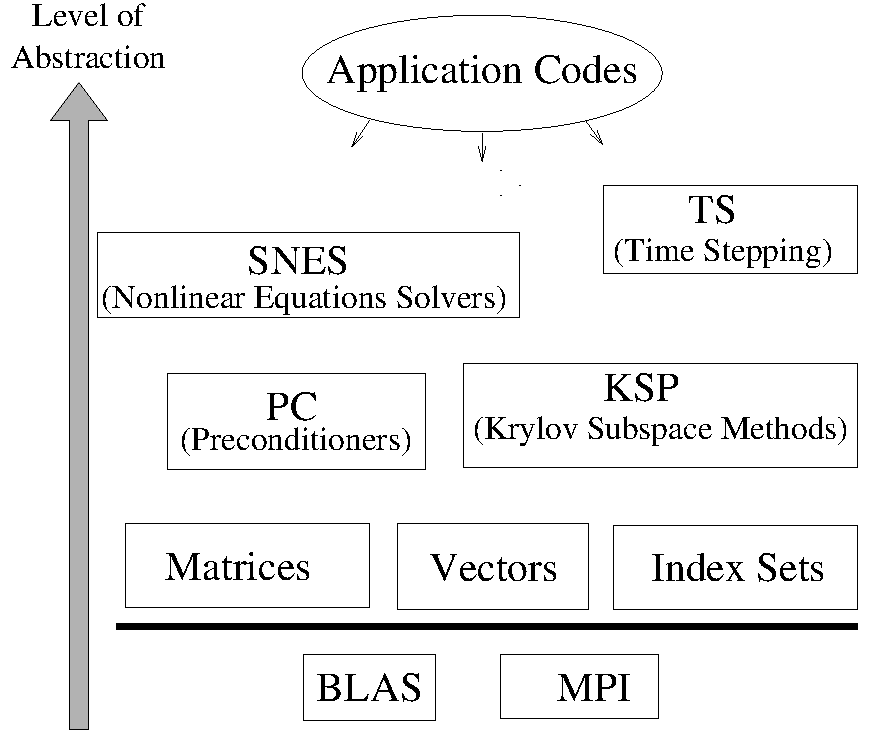
\includegraphics[scale=.5]{petscwww}
\end{numberedframe}

\begin{numberedframe}{Hierarchy of tools}
 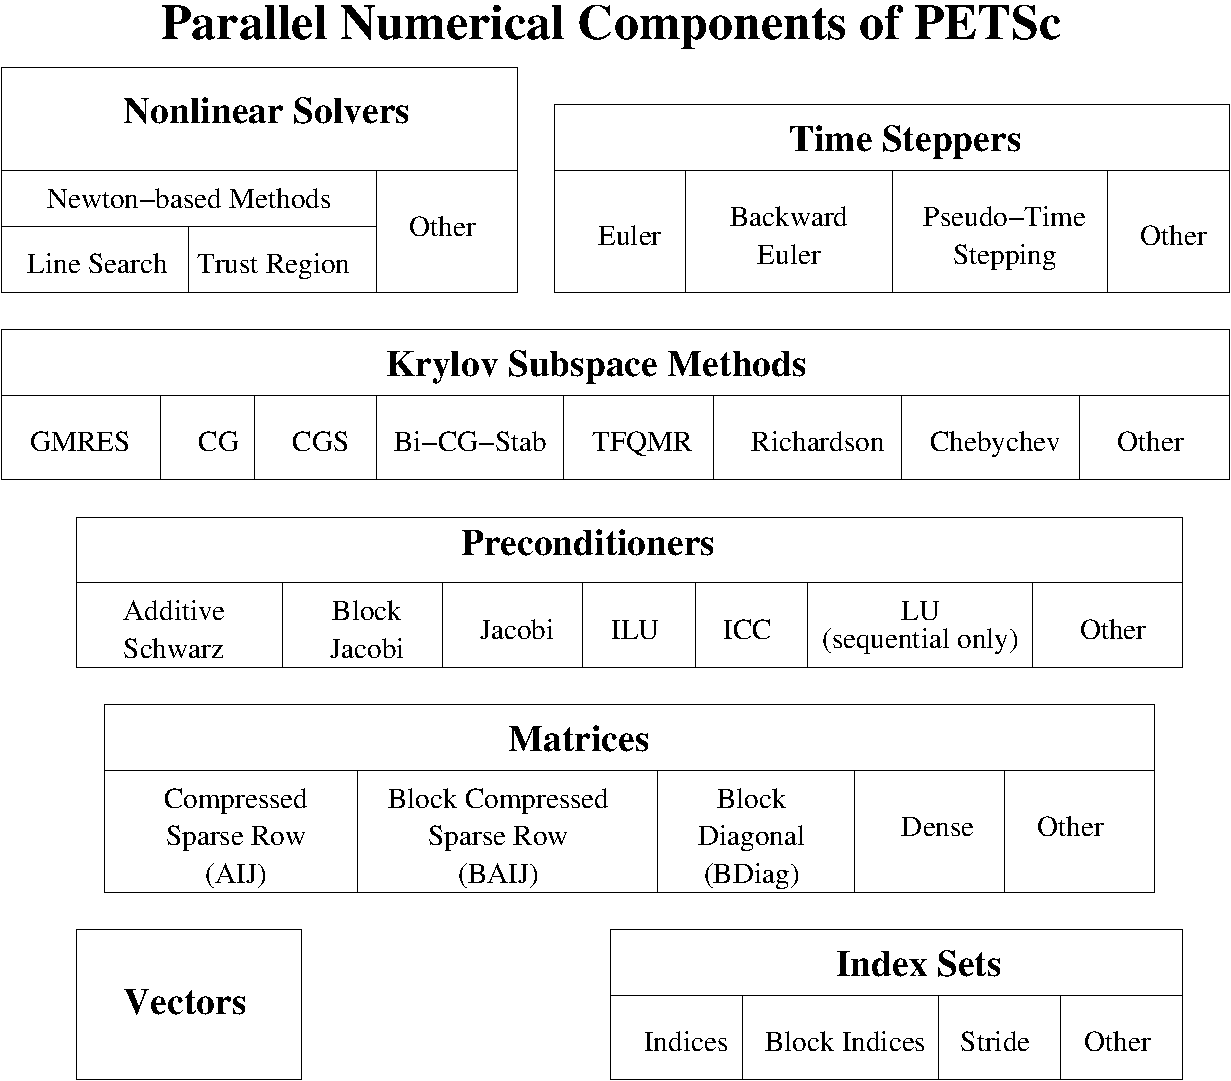
\includegraphics[scale=.45]{zoom}
\end{numberedframe}

\begin{numberedframe}{Documentation and help}
\begin{itemize}
\item Web page: \url{https://petsc.org/}
\item Documentation (pdf/html): \url{https://petsc.org/release/docs/}
\item Follow-up to this tutorial: eijkhout@tacc.utexas.edu
\item PETSc on your local cluster: ask your local support
\item General questions about PETSc: petsc-maint@mcs.anl.gov
\item Example codes, found online, and in \verb+$PETSC_DIR/src/mat/examples+
et cetera
\item Sometimes consult include files, for instance
\verb+$PETSC_DIR/include/petscmat.h+
\end{itemize}
\end{numberedframe}

\begin{details}
\begin{numberedframe}{External packages}
PETSc does not do everything, but it interfaces to other software:
  \begin{itemize}
  \item Dense linear algebra: \n{Scalapack}, \n{Plapack}, \n{Elemental}
  \item Grid partitioning software: \n{ParMetis}, \n{Jostle}, \n{Chaco}, \n{Party}
  \item ODE solvers: \n{PVODE}
  \item Optimization: \n{TAO} (now integrated)
  \item Eigenvalue solvers (including SVD): \n{SLEPc} (integrated)
  \end{itemize}
\end{numberedframe}
\end{details}

\begin{numberedframe}{PETSc and parallelism}

PETSc is layered on top of MPI

\begin{itemize}
\item
MPI has basic tools: send elementary datatypes between processors
\item PETSc has intermediate tools:\\
insert matrix element in arbitrary location,\\
do parallel matrix-vector product
\item 
$\Rightarrow$ you do not need to know much MPI when you use PETSc
\end{itemize}
\end{numberedframe}

\begin{details}
\begin{numberedframe}{PETSc and parallelism}

\begin{itemize}
\item
All objects in Petsc are defined on a communicator;\\
can only interact if on the same communicator
\item
Parallelism through MPI
\item 
  Transparent: same code works sequential and parallel.\\
  (Some objects explicitly declared \n{Seq/MPI})
\item
No OpenMP used in the library:\\
user can use shared memory programming.
\item
Likewise, threading is kept outside of PETSc code: not thread-safe.
\item Limited \ac{GPU} support; know what you're doing!
\begin{taccnote}
Only available on the Frontera RTX nodes (single precision).
\end{taccnote}
\end{itemize}

\end{numberedframe}
\end{details}

\begin{numberedframe}{Object oriented design}

Petsc uses objects: vector, matrix, linear solver, nonlinear solver

Overloading: 
\begin{verbatim}
  MATMult(A,x,y); // y <- A x
\end{verbatim}
same for sequential, parallel, dense, sparse, FFT
\end{numberedframe}

\begin{numberedframe}{Data hiding}
To support this uniform interface, the implementation is hidden:
\begin{verbatim}
  MatSetValue(A,i,j,v,INSERT_VALUES); // A[i,j] <- v
\end{verbatim}
There are some direct access routines, but most of the time you don't
need them.

(And don't worry about function call overhead.)
\end{numberedframe}
